\section{Dynamic Programming}

\subsection{Rod Cutting}

\subsubsection{Description of Problem}

\begin{itemize}
\item steel rod of length $n$, where $n$ is some integer.
\item $P[1...n]$, where $P[i]$ is market price for rod of length $i$.
\end{itemize}

\question

Suppose you can cut rod to any integer length for free.
How much money can you made?

\subsubsection{Analysis}

\begin{itemize}
\item Consider leftmost cut of optimal solution.

cut can be at positions $1...n$.

If leftmost cut at $i$, then you get $P[i]$ for leftmost piece and then optimally sell remaining $n-i$ length rod.

\item Don't know where to make first cut, so try them all and find
\[\max\left(0, \max(P[i] + cutRod(n-i))\right)\]
\end{itemize}

So, the first attempt of the algorithm could be described as \cref{cutting_rod_raw_alg}.

\begin{algorithm}[H]
\caption{First Attempt of Solving Cutting Rod Problem}\label{cutting_rod_raw_alg}
\begin{algorithmic}[1]
\Procedure{CutRod}{n}
\If{$n=0$} \Comment{If the remaining rod length is $0$.}
    \Return $0$
\EndIf
\State $q=0$
\For{$i=1 \text{ to } n$}
    \State $q = \max\left(q, P[i]+\ProcedureName{CutRod}{n-i}\right)$
\EndFor
\Return $q$
\EndProcedure
\end{algorithmic}
\end{algorithm}

Running time of \cref{cutting_rod_raw_alg}:$T(n) = n + \sum_{i=0}^{n-i}T(i)$, which is clearly \textbf{Exponential} since there are \underline{a lot of subproblem overlap}!

\subsubsection{Memoized Version}
\cref{cutting_rod_memoized_alg} illustrates the memoized version of the algorithm in \cref{cutting_rod_raw_alg}
\begin{algorithm}[H]
\caption{Memoized Version of Solving Cutting Rod Problem}\label{cutting_rod_memoized_alg}
\begin{algorithmic}[1]
\Procedure{MemRodCut}{n} \Comment{Globally define $R[1..n]$}
\If{$n=0$}
    \Return $0$
\EndIf
\If{$R[n]$ undefined}
    \State $q=0$
    \For{$i=1 \text{ to } n$}
\State $q = \max\left(q, P[i]+\ProcedureName{MemRodCut}{n-i}\right)$
    \EndFor
    \State $R[n] = q$
\EndIf
\Return $R[n]$
\EndProcedure
\end{algorithmic}
\end{algorithm}

\emph{Note that $R[1...n]$ is filled in form \underline{left to right}.} It means we can store the result and use it later, which brings us to the dynamic programming version of the algorithm.

\subsubsection{Dynamic Programming Version to Solve RodCut}
\cref{cutting_rod_dp_alg} illustrates the dynamic programming version of the algorithm according to the memoized version \cref{cutting_rod_memoized_alg}.
\begin{algorithm}[H]
\caption{Dynamic Programming Version of Solving Cutting Rod Problem}\label{cutting_rod_dp_alg}
\begin{algorithmic}[1]
\Procedure{DPRodCut}{n}
\State Let $R[0...n]$ be an array.
\State $R[0] = 0$
\For{$j = 1 \text{ to } n$}
    \State $q = 0$
    \For{$i = 0 \text{ to } j$}
        \State $q = \max(q, P[i] + R[j-i])$
    \EndFor
    \State $R[i] = q$
\EndFor
\Return $R[n]$
\EndProcedure
\end{algorithmic}
\end{algorithm}

Running time of \cref{cutting_rod_dp_alg}: $T(n) = \bigO{n^2}$.

Note that the process only computes the total number. If we are to know how to cut, we can store the cutting position during the progress.

Define $C[1...n]$, and replace the inner for loop in \cref{cutting_rod_dp_alg} as:
\begin{algorithm}[H]
\caption{Store the Cutting Position in the Process}
\begin{algorithmic}[1]
\For{$i = 0 \text{ to } j$}
    \State $q = \max(q, P[i] + R[j-i])$
    \State $C[j] = i$
\EndFor
\State $R[i] = q$
\end{algorithmic}
\end{algorithm}

The for loop does the following:
\begin{itemize}
\item $C[j]$ stores last leftmost cut length for rod of length $j$.
\item $C[n]$ says where to make first
\end{itemize}

Thus $C[n - C[n]]$ tells the second cut.

\subsection{Solving DP problem}
According to previous examples, we can summarize the general method to solve DP problem.

\begin{enumerate}
\item Write recursive solution, explain why the solution is correct.
\item Identify all subproblems considered.
\item Described how to store subproblems.
\item Find order to evaluate subproblems, s.t. subproblems you depend on evaluated \textbf{\textit{before}} current subproblem.
\item Running Time: time to fill an entry X size table.
\item Write DP/Memoized algorithm.
\end{enumerate}

\subsection{Longest Increasing Subsequence (LIS)}
\subsubsection{Description of Problem}
\AlgoInput Array $A[1...n]$ of integers.

\AlgoOutput Longest subsequence of indices, $1 \leq i_1 < i_2 < ... < i_k < n$, s.t. $A[i_j] < A[i_{j+1}]$ for all j.

Warning: Subarray is ``contiguous''. So what is a subsequence?
\begin{itemize}
    \item if $n=0$, the onl subsequence is empty sequence.
    \item otherwise, a subsequence is either
    \begin{enumerate}
        \item a subsequence of $A[2...n] or$,
        \item $A[1]$ followed by the subsequence of $A[2...n]$.
    \end{enumerate}
\end{itemize}

\subsubsection{Analysis}
Suggest recursive strategy for any array subsequence problem.
\begin{itemize}
    \item if empty, do nothing.
    \item otherwise figure out whether to take $A[1]$ and let recursion fairy handle $A[2...n]$.
\end{itemize}

However, the definition of the subsequence is not fully recursive as stated, causing handling $A[2...n]$ depends on whether take $A[1]$.

To fix it, define LIS subsequence with all elements greater than some value as follow.

\begin{itemize}
    \item LIS(prev, start) be the LIS in $A[start, n]$, s.t. all elements greater then $A[prev]$.
    \item Augment A s.t $A[0] = -\infty$, then LIS of $A[1...n]$ is LIS(0, 1).
\end{itemize}

Note that the idea of adding a $A[0]$ maybe useful in many scenarios.

\begin{algorithm}[H]
\caption{Original Algorithm for LIS Problem}\label{ori_lis_alg}
\begin{algorithmic}[1]
\Procedure{LIS}{prev, start} \Comment{$prev < start$}
\If{$start > n$}
    \Return {$0$}
\EndIf
\State $ignore = LIS(prev, start +1)$
\State best = ignore
\If{$A[start] > A[prev]$}
    \State $include = 1 + LIS(start, start+1)$
    \If{$include > ignore$}
        \State $best = include$
    \EndIf
\EndIf
\Return {$best$}
\EndProcedure
\end{algorithmic}
\end{algorithm}

\ProcedureName{LIS}{prev, start} is the length of longest increasing
subsequence in $A[start\ldots n]$, s.t. all elements greater than
$A[prev]$.

\observation

The procedure \ProcedureName{LIS}{prev, start} has the following features:

\begin{itemize}
    \item \ProcedureName{LIS}{prev, start} depends on \ProcedureName{LIS}{prev, start + 1}
    \item So need 2D table $B[0\ldots n][1\ldots n+1]$, each entry takes
        \bigO{1} time to fill in, and can fill in any ordeer,
        s.t. $B[\ ][start+1]$ filled before $B[\ ][start]$.
\end{itemize}


\subsubsection{Dynamic Programming Version to Solve LIS}
\cref{dp_lis_alg} illustrates the dp version to solve LIS problem.

\begin{algorithm}[H]
\caption{Dynamic Programming Algorithm for LIS Problem}\label{dp_lis_alg}
\begin{algorithmic}[1]
\Procedure{LISDP}{$A[1\ldots n]$}
\State $A[0] = -\infty$
\State init $B[0\ldots n][1\ldots n+1]$
\For{$i=0\text{ to }n$}
    \State $B[i][n+1]=0$
\EndFor
\For{$start = n\text{ to  }1$}
    \For{$prev = start - 1\text{ to }0$}
        \If{$A[prev] \geq A[start]$}
            \State $B[prev][start] = B[prev][start + 1]$
        \Else
        \State $B[prev][start] = \max\{(B[prev][start + 1], 1 + B[start][start + 1]\}$
        \EndIf
    \EndFor
\EndFor
\Return $B[0][1]$
\EndProcedure
\end{algorithmic}
\end{algorithm}

The running time for \cref{dp_lis_alg} is the time to fill the table, i.e. \bigO{n^2}.

\subsection{Longest Common Subsequence}

\subsubsection{Description of Problem}

\AlgoInput Character arrays: $A[1\ldots n]$, $B[1\ldots m]$.

\AlgoOutput Find length of longest common subsequence, i.e.
find length $k$ of longest pair of strings of indices.
\[1\leq i_1 < i_2 < \ldots < i_k \leq n\]
and
\[1 \leq j_1 < j_2 < \ldots < j_k \leq m\]
s.t. for all $1 \leq l \leq k$, $A[i_l] = B[j_l]$.

Example:
\begin{align*}
    A &= \{\texttt{ C G C A A T C C A G G }\} \\
    B &= \{\texttt{ G A T T A C G A }\}
\end{align*}

LCS = G A T C A.

The sequence is \{2,4,6,8,9\} and \{1,2,3,6,8\}. Note that the sequence may not be unique.

\subsubsection{Analysis}

Handle first element of A and B:
\begin{itemize}
    \item if $A$ or $B$ is empty, return $0$;
    \item if $A[1] \neq B[1]$, then $A[1]$ and $B[1]$ cannot both be used.
        So should be the best solution from throwing out $A[1]$ or $B[1]$, i.e.
%        $LCS(A[1\ldots n], B[1\ldots m]) = \max\{1+LCS(A[2\ldots n], B[2\ldots n]), LCS(A[2\ldots n], B[1\ldots m]), LCS(A[1\ldots n], B[2\ldots m])\}$

        \begin{equation}
            LCS(A[1\ldots n], B[1\ldots m]) = \max\biggl\{
                        \begin{array}{ll}
                          LCS(A[2\ldots n], B[1\ldots m]),\\
                          LCS(A[1\ldots n], B[2\ldots m])
                        \end{array}
                    \biggr\}
        \end{equation}
%    LCS(A[1\ldots n], B[1\ldots m]) = \max\{& LCS(A[2\ldots n], B[1\ldots m]),\\
%                                            & LCS(A[1\ldots n], B[2\ldots m])\}
    \item if $A[1] = B[1]$, then can either match or throw both of them out, i.e
        \begin{equation}
            LCS(A[1\ldots n], B[1\ldots m]) = \max\Biggl\{
                        \begin{array}{ll}
                          1+LCS(A[2\ldots n], B[2\ldots n]),\\
                          LCS(A[2\ldots n], B[1\ldots m]),\\
                          LCS(A[1\ldots n], B[2\ldots m])
                        \end{array}
                    \Biggr\}
        \end{equation}
%    LCS(A[1\ldots n], B[1\ldots m]) = \max\{& 1+LCS(A[2\ldots n], B[2\ldots n]),\\
%                                            & LCS(A[2\ldots n], B[1\ldots m]),\\
%                                            & LCS(A[1\ldots n], B[2\ldots m])\}
\end{itemize}

Note that if $A[1] = B[1]$, why consider throw them out?

Though without proof, the option is right, but generally,
the option should be considered.

The algorithm is described in \cref{ori_lcs_alg}.
\ProcedureName{LCS}{curA, CurB} is the longest common sequence of
$A[curA \ldots n]$ and $B[curB \ldots m]$.
\begin{algorithm}[H]
\caption{Original Algorithm for LCS Problem}\label{ori_lcs_alg}
\begin{algorithmic}[1]
    \Procedure{LCS}{$curA, curB$}
        \If{$curA > n$ or $ curB > m$}
            \Return $0$
        \EndIf
        \State $ignore = \max\{LCS(curA+1, CurB), LCS(CurA, CurB+1)\}$
        \State $best = ignore$
        \If{$A[curA] = B[curB]$}
            \State $include = 1 + LCS(curA+1, curB+1)$
            \If{$include > ignore$}
                \State $best = include$
            \EndIf
        \EndIf
        \Return $best$
    \EndProcedure
\end{algorithmic}
\end{algorithm}

To find LCS of $A[1 \ldots n]$, $B[1 \ldots m]$, call \ProcedureName{LCS}{1,1}.

\observation

The procedure \ProcedureName{LCS}{curA, curB} has the following features:

\begin{itemize}
    \item \ProcedureName{LCS}{curA, curB} depends on two parameters,
        need a 2D array of total size \bigO{nm}.
    \item \ProcedureName{LCS}{curA, curB} makes 3 recursive calls.
        All recursive calls have at least one parameter strictly
        larger, and none smaller.
    \item The table can be filled in two nested decreasing for loop.
\end{itemize}

\subsubsection{Dynamic Programming Version to Solve LCS}

The DP algorithm to solve LCS problem is showed in \cref{dp_lcs_alg}.


\begin{algorithm}[H]
\caption{Dynamic Programming Algorithm for LCS Problem}\label{dp_lcs_alg}
\begin{algorithmic}[1]
    \Procedure{LCSDP}{$A[1 \ldots n], B[1 \ldots m]$}
        \State Define $C[1 \ldots n+1][1 \ldots m+1]$
        \For{$i=0\text{ to }n+1$}
            \State $C[i][m+1]=0$
        \EndFor
        \For{$i=0\text{ to }m+1$}
            \State $C[n+1][i]=0$
        \EndFor
        \For{$curA = n\text{ to }1$}
            \For{$curB = m\text{ to }1$}
                \State $ignore = \max\{C[curA+1][CurB], C[curA][curB+1]\}$
                \State $best = ignore$
                \If{$A[curA] = B[curB]$}
                    \State $include = 1 + C[curA+1][curB+1]$
                    \If{$include > ignore$}
                        \State $best = include$
                    \EndIf
                \EndIf
                \State $C[curA][curB] = best$
            \EndFor
        \EndFor
        \Return $C[1][1]$
    \EndProcedure
\end{algorithmic}
\end{algorithm}

The operation to fill the table takes \bigO{1} time, ignoring recursive calls.

So, total time is $\bigO{n\times m\times 1} = \bigO{nm}$.

\subsection{Edit Distance}

\subsubsection{Description of Problem}

\AlgoInput Character arrays: $A[1 \ldots m]$, $B[1 \ldots n]$

\AlgoOutput Edit distance between $A$ and $B$, which is the minimum number
of characters insertion, deletion and substitution to turn $A$ into $B$.

\AlgoExample For character arrays $A$ and $B$:

\begin{align*}
    A &= \{\texttt{ F O O D }\} \\
    B &= \{\texttt{ M O N E Y }\}
\end{align*}

The edit process is:

\begin{align*}
    \texttt{F O O D} &\rightarrow \texttt{M O O D} \\
                     &\rightarrow \texttt{M O N D} \\
                     &\rightarrow \texttt{M O N E D} \\
                     &\rightarrow \texttt{M O N E Y}
\end{align*}

\subsubsection{Analysis}

Consider a better way to display edits:

Place $A$ above $B$, put a gap in $A$ for each insertion, gap in $B$ for
each deletion, i.e.

\begin{align*}
    A &= \{\texttt{ F O O \ \ D }\} \\
    B &= \{\texttt{ M O N E Y }\}
\end{align*}

Then, the edit distance is the number of columns where characters don't
match (in an optional alignment).

Let $edit(A, B)$ denotes the edit distance from $A$ to $B$.
Note that $edit(A, B) = edit(B, A)$.

Another example:

\begin{align*}
    A &= \{\texttt{A\ L\  G\ O\ R\ \ \ I\ \ \ T\ H\ M }\} \\
    B &= \{\texttt{A\ L\ \ \ T\ R\ U\  I\  S\ T\ I\ C }\}
\end{align*}


If remove last column from an optimal alignment,
the remaining must represent the shortest edit sequence
for remaining substrings.

So now we can recursively define edit distance $edit(A, B)$:
\begin{itemize}
    \item if $m = 0$, i.e. $A$ is empty, then $edit(A, B) = n$;
    \item if $n = 0$, i.e. $B$ is empty, then $edit(A, B) = m$;
    \item otherwise, $m,n \geq 1$, then look at last column in optimal alignment.
        There are three cases:
        \begin{enumerate}[label=\alph*)]
            \item insertion, i.e. top row empty, which means:
                \begin{itemize}
                    \item All of $A$ remains to left;
                    \item All but last character of $B$ to left;
                \end{itemize}
                \[edit(A[1 \ldots m], B[1 \ldots n]) = edit(A[1 \ldots m], B[1 \ldots n-1]) + 1\]
            \item deletion, i.e. bottom row empty, which means, like insertion:
                \[edit(A[1 \ldots m], B[1 \ldots n]) = edit(A[1 \ldots m-1], B[1 \ldots n]) + 1\]
            \item substitution, i.e. both rows non-empty, which means:
                \[edit(A[1 \ldots m], B[1 \ldots n]) = edit(A[1 \ldots m-1], B[1 \ldots n-1]) + [A[m] \neq B[n]]\]
                where the condition $[A[m] \neq B[n]]$ is $1$ if true and $0$ if false.
        \end{enumerate}
\end{itemize}

The algorithm is described in \cref{ori_edit_distance}.
$\ProcedureName{Edit}{i, j} = edit(A[1 \ldots i], B[1 \ldots j])$.

\begin{algorithm}[H]
    \caption{Original Algorithm for Edit Distance}\label{ori_edit_distance}
    \begin{algorithmic}
        \Procedure{Edit}{$i,j$}
            \If{$i = 0$}
                \Return $j$
            \EndIf
            \If{$j = 0$}
                \Return $i$
            \EndIf
            \Return $\min\{\ProcedureName{Edit}{i-1,j}+1,\ProcedureName{Edit}{i,j-1}+1,\ProcedureName{Edit}{i-1,j-1}+[A[i]\neq B[j]]\}$
        \EndProcedure
    \end{algorithmic}
\end{algorithm}

\observation

The procedure \ProcedureName{Edit}{i,j} has the following features:

\begin{itemize}
    \item $i$ has $m$ values.
    \item $j$ has $n$ values.
    \item store in table of size \bigO{mn}.
    \item \ProcedureName{Edit}{i,j} depends on three sub-problems,
        in each case either $i$ or $j$ smaller (and never larger).
    \item can fill in table with two nested increasing for loop.
    \item constant time per entry, so \bigO{mn} overall.
\end{itemize}

\subsubsection{Dynamic Programming Version to Solve Edit Distance Problem}

The DP algorithm to solve Edit Distance problem is showed in \cref{dp_edit_distance}.

\begin{algorithm}[H]
\caption{Dynamic Programming Algorithm for Edit Distance Problem}\label{dp_edit_distance}
\begin{algorithmic}[1]
    \Procedure{EditDP}{$A[i \ldots m], B[i \ldots n]$}
        \For{$j=0\text{ to }n$}
            \State $E[0][j]=j$
        \EndFor
        \For{$i=0\text{ to }n$}
            \State $E[i][0]=i$
        \EndFor
        \For{$i = 1\text{ to }m$}
            \For{$j = 1\text{ to }n$}
                \If{$A[i] = B[j]$}
                    \State $E[i][j] = \min\{E[i-1][j]+1, E[i][j-1]+1, E[i-1][j-1]\}$
                \Else
                    \State $E[i][j] = \min\{E[i-1][j]+1, E[i][j-1]+1, E[i-1][j-1]+1\}$
                \EndIf
            \EndFor
        \EndFor
        \Return $E[m][n]$
    \EndProcedure
\end{algorithmic}
\end{algorithm}

The operation to fill the table takes \bigO{1} time, ignoring recursive calls.

So, total time is obviously \bigO{mn}.

\subsection{Longest Convex Subsequence}

\subsubsection{Description of Problem}

\AlgoInput Array $A[1\ldots n]$ of integers.

\AlgoOutput Longest subsequence of indices,
\[1 \leq i_1 < i_2 < ... < i_k < n\]
s.t. $2\times A[i_j] < A[i_{j-1}] + A[i_{j+1}]$ for all j.

\subsubsection{Analysis}
If consider $A[i]$ as current element, whether choose it or throw it depends on its
next element. Thus, consider $A[i+1]$ as current element.

\begin{algorithm}[h]
    \caption{Recursive Algorithm for Longest Convex Subsequence}\label{ori_lxs_alg}
    \begin{algorithmic}[1]
        \Procedure{LXS}{$preprev, prev, cur$}
            \If{$cur > n$}
                \Return $0$
            \EndIf
            \State $ignore = $\ProcedureName{LXS}{\tikzmark[red]{point1}{\underline{$preprev, prev$}}, \tikzmark[blue]{point2}{\underline{$cur+1$}}}
            \State $best = ignore$
            \If{$preprev = -1$ or $A[cur] > 2\times A[prev] - A[preprev]$}
                \State $include = 1 + \ProcedureName{LXS}{prev, cur, cur+1}$
                \If{$include>ignore$}
                    \State $best = include$
                \EndIf
            \EndIf
            \Return $best$
        \EndProcedure
    \end{algorithmic}
    
    \begin{tikzpicture}[remember picture,overlay,node distance = 1cm]
        \node[red] (point1descr) [above right =of point1]{Does not change.};
        \draw[red,->,thick] (point1descr) to [in=45,out=-135] (point1);
        \node[blue] (point2descr) [right =of point2]{Consider next element.};
        \draw[blue,->,thick] (point2descr) to [in=-30,out=-150] (point2);
    \end{tikzpicture}
\end{algorithm}

Call \ProcedureName{LXS}{-1,-1,1} will get the longest convex sequence.

There are three parameter with $n$ size, so the table is \bigO{n^3} size.

Each entry require \bigO{1} time to fill, so the total running time is \bigO{n^3}.

The third parameter $cur$ is always strictly larger, so the outer for loop
should be a decreasing for loop for $cur$. The inner two for loop is irrelevant.

\subsection{Professor's note on LIS/LCS/LXS/SCS}

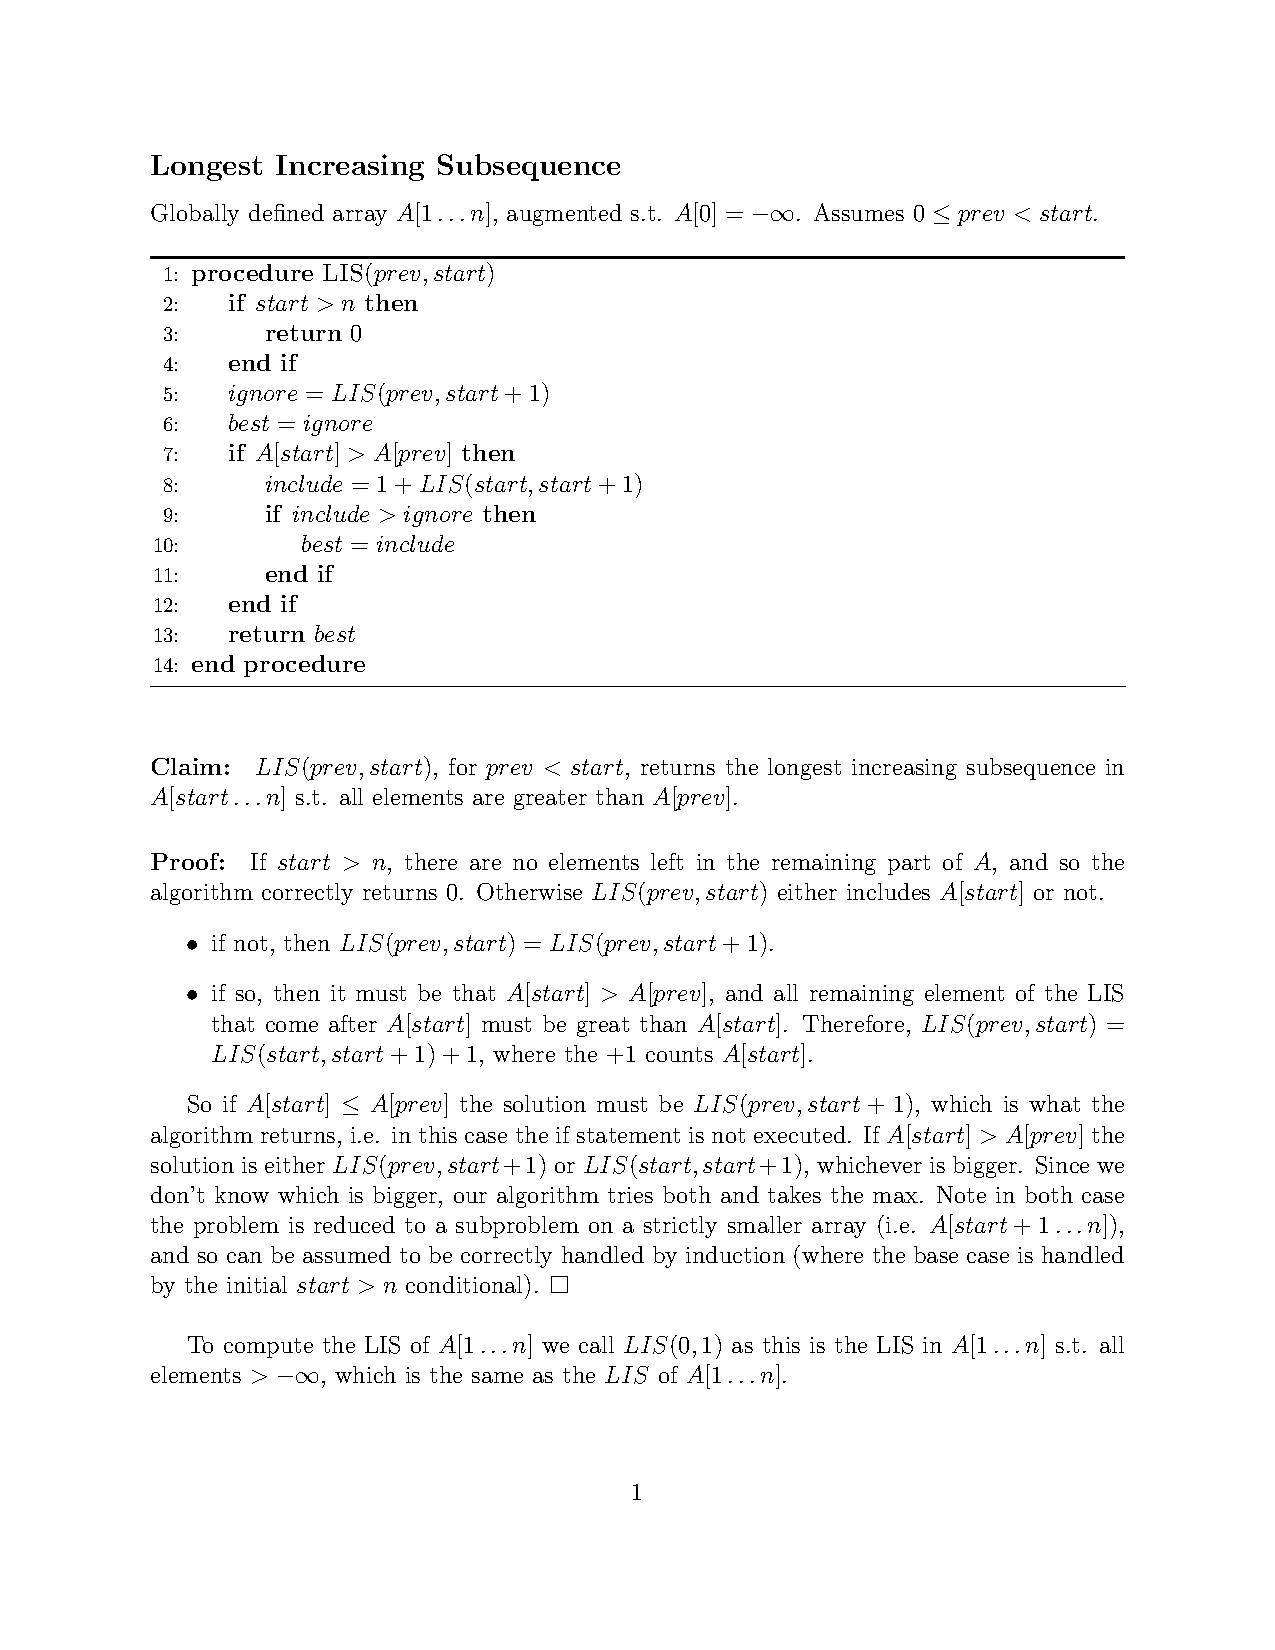
\includepdf[pages=-]{lis.pdf}
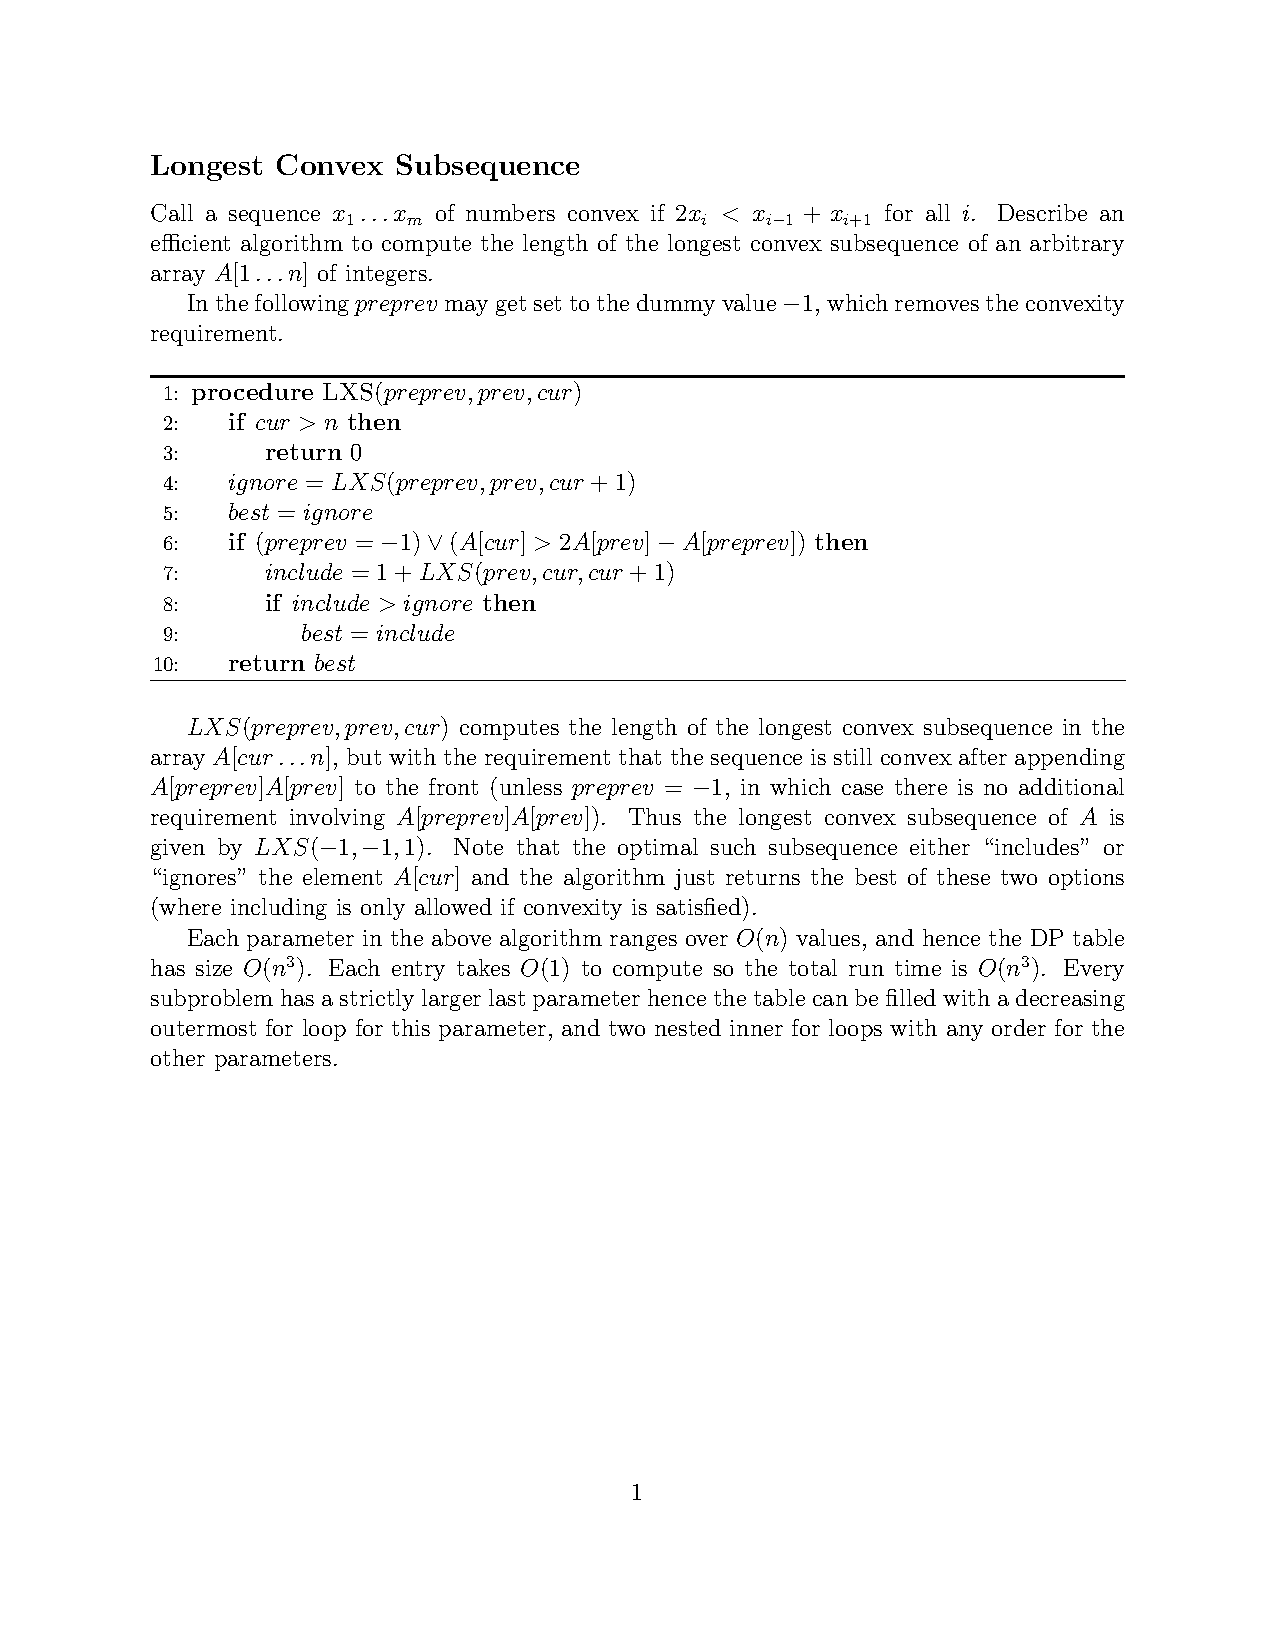
\includepdf[pages=-]{lxs.pdf}

\subsection{Summary}

Quote from professor:

\begin{quote}

When solving the DP problem on the exam ask yourself:

\begin{quote}
``What is the minimal amount of information needed to
determine whether I can take the current element as the
next element in the subsequence?''
\end{quote}

For the longest convex subsequence I need to know what the
previous two elements in the subsequence were. Shortest
common super-sequence was even easier, as there is no
requirement imposed by earlier elements. In both problems
we then try all options of taking or not taking the current
element(s) and return the best result.

\end{quote}

For increasing/decreasing in the For-Loop, look for the parameter(s)
that is strictly increasing or decreasing.
\begin{itemize}
    \item If only one is increasing/decreasing, then the outer For-Loop should
        be decreasing/increasing about that parameter.
        The other For-Loop is irrelevant (for example the inner two For-Loop in LXS).
    \item If both parameter is increasing/decreasing, then two For-Loop should
        both be decreasing/increasing about its parameter. Which For-Loop
        is the outer one is irrelevant (for example the two For-Loop in SCS).
\end{itemize}
